%!TEX program = xelatex
\let\stop\empty

\documentclass[12pt,a4paper]{exam-zh}

\usepackage{xeCJK}
% \setCJKmainfont{NSimSun}
\setCJKmainfont{Noto Serif CJK SC}
\usepackage{geometry}
\usepackage{array}
\usepackage{tikz}
\usepackage{amsmath}
\usepackage{wrapfig}
\usepackage{adjustbox}
\usepackage{enumitem}
\usepackage{fancyhdr}
\usetikzlibrary{quotes,angles}
\usepackage{scalerel}
\def\mcirc{\mathbin{\scalerel*{\circ}{j}}}
\def\msquare{\mathord{\scalerel*{\Box}{gX}}}

% \renewcommand{\choiceshook}{%
%     \setlength{\leftmargin}{18pt}%
% }
\geometry{margin=2cm}



%region ----------- 调整 exam -----------
\examsetup{
    % problem/label = \arabic*., 
    % 设置大题题号格式 
        problem = {
        top-sep = 1em,      % 题头上方的间距（默认 0.25em）
        bottom-sep = 1em,   % 题号下方的间距（默认 0pt）
    },
    % 隐藏大题后的分值显示 
    problem/show-points = false,
    question = {
        top-sep = 1em,
        bottom-sep = 1em,
    },
    % 调整小题列表的缩进和间距
    list/step-name = {}, 
    solution = {
    show-solution = show-move, % 答案自动移动到卷末
    label-content = {参考答案},  % 答案区的标题文字
    show-qed = true            % 在解答末尾显示结束符号 ◻ 
  },
    page = {
    size = a4paper,           % 设定纸张大小 
    foot-content = { - ; - }  % 页脚显示为 -1-, -2- 格式 
  }
}
\setlist[enumerate,1]{
    label=(\alpha*), 
    itemsep=0.5em, 
    leftmargin=2em, 
    after=\hfill % 配合您之前要求的百分比靠右样式
}
\newlist{questionparts}{enumerate}{1}
\setlist[questionparts]{
    label=(\alph*),
    itemsep=0.5em,
    leftmargin=2em,
    rightmargin=4em
}
\newcommand{\qscore}[1]{%
    \unskip\nobreak\hfill
    \makebox[0pt][l]{\makebox[4em][r]{(#1\%)}}%
}
%endregion


% ==========================
% 卷面变量设置（只需改这里）
% ==========================
% ==========================
% 卷面变量设置（只需改这里）
% ==========================
\newcommand{\paperlevel}{高中一文商班}
\newcommand{\papersubject}{数学（试卷二）}
\newcommand{\schoolname}{金宝培元独立中学}
\newcommand{\examname}{八月考}
\newcommand{\classinfo}{S1(Y / H)}
\newcommand{\examdate}{6-8-2026}
\newcommand{\examtime}{11:00-12:15}
\newcommand{\questiontotal}{5}
\newcommand{\paperpercentage}{50\%}
\newcommand{\setterteacher}{蔡杰庆师}
\newcommand{\reviewteacher}{王萌师}
\newcommand{\auditteacher}{雷泳健师}

\begin{document}


%region 三栏标题区
% ==========================
\noindent
\begin{tabular*}{\textwidth}{@{\extracolsep{\fill}} p{0.3\textwidth} p{0.35\textwidth} p{0.3\textwidth}}

\raggedright
\textbf{\paperlevel}\\[0.2em]
\textbf{}{\papersubject}\\[0.4em]
姓名：\underline{\hspace{3cm}} &

\centering
\textbf{\schoolname}\\[0.2em]
\textbf{\examname}\\[0.4em]
班级：\classinfo &

\raggedright
日期：\examdate\\[0.2em]
时间：\examtime\\[0.4em]
得分：\underline{\hspace{2.5cm}} \\

\end{tabular*}

\begin{flushleft}
作答题：\questiontotal 题全做（\paperpercentage） 
\end{flushleft}
%endregion

% %region 范围：高中数学 - 线性规划 | 考点：线性规划、约束条件建立、可行区域、目标函数最优值 | 难度：中等
% \begin{question}[points = 10]
%     某工厂计划生产两种产品 $A$ 与 $B$。已知生产每单位产品 $A$ 需耗用机器时间 $2$ 小时及原料 $1$ 单位；生产每单位产品 $B$ 需耗用机器时间 $1$ 小时及原料 $3$ 单位。该厂每日可用机器时间上限为 $10$ 小时，原料供应上限为 $15$ 单位。设该厂每日生产产品 $A$ 为 $x$ 单位，产品 $B$ 为 $y$ 单位。若每售出一单位产品 $A$ 可获利 $3$ 元，每售出一单位产品 $B$ 可获利 $5$ 元。

%     \begin{questionparts}
%         \item 根据上述条件，列出所有约束条件及目标函数 $P$。 \qscore{4}

%         \item 承 (a)，在坐标平面上画出满足所有约束条件的可行区域 $R$，并清楚标示各边界直线与顶点坐标。 \qscore{6}

%         \item 利用 (b) 中所绘之可行区域 $R$，求该厂每日可获得的最大利润，并指出达到最大利润时 $x$ 与 $y$ 的值。 \qscore{3}
%     \end{questionparts}
% \end{question}

% \begin{solution}
%     \begin{enumerate}[label=(\alph*)]
%         \item \textbf{列出约束条件及目标函数：} \\
%         由机器时间限制：每单位 $A$ 耗时 $2$ 小时、每单位 $B$ 耗时 $1$ 小时，上限为 $10$ 小时，得 \\
%         $2x + y \leq 10$ \hfill (1分) \\
%         由原料供应限制：每单位 $A$ 耗料 $1$ 单位、每单位 $B$ 耗料 $3$ 单位，上限为 $15$ 单位，得 \\
%         $x + 3y \leq 15$，并由生产量不为负，得 $x \geq 0,\ y \geq 0$ \hfill (1分) \\
%         每日利润为售出两产品所得之和，故目标函数为 \\
%         $P = 3x + 5y$ \hfill (1分)

%         \item \textbf{绘出可行区域：} \\
%         先求各边界直线与坐标轴的交点，以便绘图： \\
%         直线 $2x + y = 10$：与 $x$ 轴交于 $(5, 0)$，与 $y$ 轴交于 $(0, 10)$ \\
%         直线 $x + 3y = 15$：与 $x$ 轴交于 $(15, 0)$，与 $y$ 轴交于 $(0, 5)$ \hfill (2分) \\
%         由 $2x + y \leq 10$ 及 $x + 3y \leq 15$ 可知可行区域应取两直线靠近原点一侧，并结合 $x \geq 0,\ y \geq 0$，正确判断方向并绘出阴影区域 $R$，其顶点为 $(0,0)$、$(5,0)$、$(3,4)$、$(0,5)$： \hfill (2分)

%         \begin{tikzpicture}[scale=0.6, >=stealth]
%             \draw[step=1cm, gray!30, very thin] (-1,-1) grid (7,7);

%             \fill[blue!15] (0,0) -- (5,0) -- (3,4) -- (0,5) -- cycle;

%             \draw[thick, blue!70!black] (0,10) -- (5,0);
%             \draw[thick, red!70!black] (0,5) -- (15,0);
%             \draw[thick] (0,0) -- (0,5);
%             \draw[thick] (0,0) -- (5,0);

%             \draw[->, thick] (-1, 0) -- (7, 0) node[right] {$x$};
%             \draw[->, thick] (0, -1) -- (0, 7) node[above] {$y$};

%             \filldraw (0,0) circle (2pt) node[below left] {$(0,0)$};
%             \filldraw (5,0) circle (2pt) node[below right] {$(5,0)$};
%             \filldraw (3,4) circle (2pt) node[above right] {$(3,4)$};
%             \filldraw (0,5) circle (2pt) node[above left] {$(0,5)$};
%             \node[below left] at (0,0) {$O$};
%         \end{tikzpicture}

%         \item \textbf{求最大利润：} \\
%         将 (b) 中可行区域 $R$ 的各顶点坐标代入目标函数 $P = 3x + 5y$： \\
%         $(0,0)$：$P = 3(0) + 5(0) = 0$ \\
%         $(5,0)$：$P = 3(5) + 5(0) = 15$ \\
%         $(3,4)$：$P = 3(3) + 5(4) = 29$ \\
%         $(0,5)$：$P = 3(0) + 5(5) = 25$ \hfill (1分) \\
%         比较以上各值，可知 $P$ 的最大值在顶点 $(3, 4)$ 处取得，最大值为 $29$。 \hfill (1分) \\
%         \textbf{答：当 $x = 3$、$y = 4$ 时，该厂每日可获得最大利润 $29$ 元。} \hfill (1分)
%     \end{enumerate}
% \end{solution}
% %endregion

%region 范围：高中数学-线性规划 | 考点：图解法求可行域与目标函数最值 | 难度：中等
\begin{question}[points = 10]
    已知变量 $x,y$ 满足以下不等式组：
    \[
    \begin{cases}
        x \geq 0 \\
        y \geq 0 \\
        x + y \leq 6 \\
        2x + y \leq 8
    \end{cases}
    \]

    \begin{questionparts}
        \item 在坐标纸上画出满足上述不等式组的可行区域。 \qscore{6}

        \item 求目标函数 $z = 3x + 2y$ 的最大值。 \qscore{4}
    \end{questionparts}
\end{question}

\begin{solution}
    \begin{enumerate}[label=(\alph*)]
        \item 画出满足不等式组 $x\geq0,\ y\geq0,\ x+y\leq6,\ 2x+y\leq8$ 的可行区域。 \\
        分别绘出各边界直线并取交集所在阴影部分。
        \begin{center}
            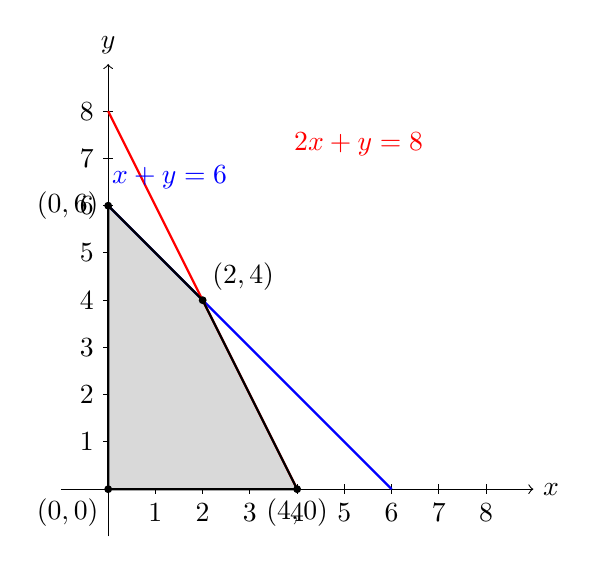
\begin{tikzpicture}[scale=0.6]
                \draw[->] (-1,0) -- (9,0) node[right] {$x$};
                \draw[->] (0,-1) -- (0,9) node[above] {$y$};
                \foreach \x in {1,...,8} \draw (\x,0.1) -- (\x,-0.1) node[below] {\x};
                \foreach \y in {1,...,8} \draw (0.1,\y) -- (-0.1,\y) node[left] {\y};

                \fill[gray!30] (0,0) -- (4,0) -- (2,4) -- (0,6) -- cycle;

                \draw[thick, blue] (0,6) -- (6,0);
                \draw[thick, red] (0,8) -- (4,0);

                \draw[thick] (0,0) -- (4,0) -- (2,4) -- (0,6) -- cycle;

                \filldraw (0,0) circle (2pt) node[below left] {$(0,0)$};
                \filldraw (4,0) circle (2pt) node[below] {$(4,0)$};
                \filldraw (2,4) circle (2pt) node[above right] {$(2,4)$};
                \filldraw (0,6) circle (2pt) node[left] {$(0,6)$};

                \node[blue] at (1.3,6.6) {$x+y=6$};
                \node[red] at (5.3,7.3) {$2x+y=8$};
            \end{tikzpicture}
        \end{center}
        \hfill (1分：直线 $x+y=6$ 正确) \\
        \hfill (1分：直线 $2x+y=8$ 正确) \\
        \hfill (1分：阴影区域正确) \\
        \hfill (1分：交点 $(4,0),(2,4),(0,6)$ 标注正确)

        \item 求 $z = 3x+2y$ 在可行区域上的最大值。 \\
        目标函数的最值在可行区域的顶点处取得，逐一代入各顶点坐标。
        \begin{align*}
            (0,0): \quad z &= 3(0) + 2(0) = 0 \\
            (4,0): \quad z &= 3(4) + 2(0) = 12 \\
            (2,4): \quad z &= 3(2) + 2(4) = 14 \\
            (0,6): \quad z &= 3(0) + 2(6) = 12
        \end{align*}
        \hfill (4分：四个顶点代入计算各得 1 分) \\
        比较各顶点所得 $z$ 值，最大值在 $(2,4)$ 处取得。
        \[
            z_{\max} = 14
        \]
        \hfill (2分)
    \end{enumerate}
\end{solution}
%endregion

%region 范围：高中数学 - 函数 | 考点：复合函数、逆推函数表达式、复合函数相等方程 | 难度：中等
\begin{question}[points = 15]
    设 $f$ 与 $g$ 为定义在实数集上的函数，$(f \circ g)(x)$ 表示先以 $g$ 作用于 $x$，再以 $f$ 作用于所得结果，即 $(f \circ g)(x) = f(g(x))$。

    \begin{questionparts}
        \item 已知 $f(x) = 3x - 5$，且 $(f \circ g)(x) = 3x^2 - 2$，求 $g(x)$。 \qscore{4}

        \item 已知 $g(x) = 2x + 3$，且 $(g \circ f)(x) = 2x^2 - 4x + 7$，求 $f(x)$。 \qscore{5}

        \item 已知 $f(x) = x + 2$ 且 $g(x) = x^2 - 1$，求$m$的值使得 $(f \circ g)(m) = (g \circ f)(m)$。 \qscore{5}
    \end{questionparts}
\end{question}

\begin{solution}
    \begin{enumerate}[label=(\alph*)]
        \item \textbf{求 $g(x)$：} \\
        由复合函数定义，$(f \circ g)(x) = f(g(x)) = 3g(x) - 5$ \hfill (1分) \\
        依题意，此式应等于 $3x^2 - 2$，故列方程： \\
        $3g(x) - 5 = 3x^2 - 2$ \hfill (2分) \\
        整理得 $3g(x) = 3x^2 + 3$，两边除以 $3$： \\
        $g(x) = x^2 + 1$ \hfill (2分) \\
        \textbf{答：$g(x) = x^2 + 1$。}

        \item \textbf{求 $f(x)$：} \\
        由复合函数定义，$(g \circ f)(x) = g(f(x)) = 2f(x) + 3$ \hfill (1分) \\
        依题意，此式应等于 $2x^2 - 4x + 7$，故列方程： \\
        $2f(x) + 3 = 2x^2 - 4x + 7$ \hfill (2分) \\
        整理得 $2f(x) = 2x^2 - 4x + 4$，两边除以 $2$： \\
        $f(x) = x^2 - 2x + 2$ \hfill (2分) \\
        \textbf{答：$f(x) = x^2 - 2x + 2$。}

        \item \textbf{求 $m$ 值：} \\
        分别求出 $(f \circ g)(m)$ 与 $(g \circ f)(m)$ 的表达式： \\
        $(f \circ g)(m) = f(g(m)) = f(m^2 - 1) = (m^2 - 1) + 2 = m^2 + 1$ \\
        $(g \circ f)(m) = g(f(m)) = g(m + 2) = (m + 2)^2 - 1 = m^2 + 4m + 3$ \hfill (2分) \\
        令两式相等，列方程： \\
        $m^2 + 1 = m^2 + 4m + 3$ \hfill (2分) \\
        两边消去 $m^2$ 项，得 $1 = 4m + 3$，解得 $m = -\dfrac{1}{2}$ \hfill (1分) \\
        \textbf{答：$m = -\dfrac{1}{2}$。}
    \end{enumerate}
\end{solution}
%endregion

%region 范围：高中数学 - 函数 | 考点：函数的定义域与值域、分式函数的反函数 | 难度：基础
\begin{question}[points = 12]
    \begin{questionparts}
        \item 已知函数 $f(x) = \sqrt{4 - x^2}$，求 $f$ 的定义域 $D_f$ 与值域。 \qscore{4}

        \item 已知函数 $f(x) = \dfrac{2x + 1}{x - 3}$，$x \neq 3$，求其反函数 $f^{-1}(x)$，并写出 $f^{-1}$ 的定义域。 \qscore{6}
    \end{questionparts}
\end{question}

\begin{solution}
    \begin{enumerate}[label=(\alph*)]
        \item \textbf{求定义域与值域：} \\
        由于根号内的值不可为负，故须满足： \\
        $4 - x^2 \geq 0$ \hfill (1分) \\
        解此不等式：$x^2 \leq 4$，即 $-2 \leq x \leq 2$ \hfill (1分) \\
        $\therefore D_f = [-2, 2]$ \hfill (1分) \\
        对于值域，由 $-2 \leq x \leq 2$ 可知 $0 \leq 4 - x^2 \leq 4$ \hfill (2分) \\
        两边开根号（根号为非负函数），得 $0 \leq \sqrt{4 - x^2} \leq 2$，即 $0 \leq f(x) \leq 2$ \\
        $\therefore$ 值域为 $[0, 2]$ \hfill (1分)

        \item \textbf{求反函数：} \\
        设 $y = f(x) = \dfrac{2x + 1}{x - 3}$ \\
        交叉相乘，去分母： \\
        $y(x - 3) = 2x + 1$ \\
        $xy - 3y = 2x + 1$ \hfill (2分) \\
        将含 $x$ 的项移至同一边，整理： \\
        $xy - 2x = 1 + 3y$ \\
        $x(y - 2) = 3y + 1$ \\
        $x = \dfrac{3y + 1}{y - 2}$ \hfill (2分) \\
        将 $x$ 与 $y$ 互换，得反函数： \\
        $f^{-1}(x) = \dfrac{3x + 1}{x - 2}$，其定义域为 $x \neq 2$ \hfill (2分) \\
        \textbf{答：$f^{-1}(x) = \dfrac{3x + 1}{x - 2}$，定义域为 $\{x \mid x \neq 2\}$。}
    \end{enumerate}
\end{solution}
%endregion

% %region 范围：高中数学 - 弧度制 | 考点：弧度制、扇形与弓形（circular segment）面积 | 难度：中等
% \begin{question}[points = 12]
%     如图所示，$OAB$ 为一直角三角形，其中 $\angle AOB = 90°$，$OA = 5$ cm，$OB = 12$ cm。弧 $AC$ 的圆心为 $O$，点 $C$ 在 $AB$ 上。
% \begin{center}
%       \begin{tikzpicture}[scale=0.7, >=stealth]
%         \coordinate (O) at (0,0);
%         \coordinate (A) at (0,5);
%         \coordinate (B) at (12,0);
%         \coordinate (C) at (3.5503,3.5207);

%         \fill[orange!60] (A) -- (C) arc (44.76:90:5) -- cycle;

%         \draw[thick] (O) -- (A) -- (B) -- cycle;
%         \draw[thick, dashed] (O) -- (C);
%         \draw[thick] (A) arc (90:44.76:5);

%         \pic [draw, angle radius=3mm] {right angle = A--O--B};

%         \node[left] at (0,2.5) {$5$ cm};
%         \node[below] at (6,0) {$12$ cm};
%         \node[above] at (A) {$A$};
%         \node[below left] at (O) {$O$};
%         \node[below right] at (B) {$B$};
%         \node[right] at (C) {$C$};
%     \end{tikzpicture}

% \end{center}

%     \begin{questionparts}
%         \item 求 $\angle AOC$，答案以弧度表示。 \qscore{6}
%         \item 求着色部分（弓形 $AC$）的面积。 \qscore{6}
%     \end{questionparts}
% \end{question}

% \begin{solution}
%     \begin{enumerate}[label=(\alph*)]
%         \item \textbf{求 $\angle AOC$：} \\
%         在直角三角形 $OAB$ 中，$\angle AOB = 90°$，利用毕氏定理求 $AB$： \\
%         $AB^2 = OA^2 + OB^2 = 5^2 + 12^2 = 169 \implies AB = 13$ cm \hfill (1分) \\
%         求 $\angle OAB$： \\
%         $\cos(\angle OAB) = \dfrac{OA}{AB} = \dfrac{5}{13}$ \\
%         $\angle OAB = \cos^{-1}\left(\dfrac{5}{13}\right) = 1.176$ rad（4 位有效数字） \hfill (2分) \\
%         由于弧 $AC$ 的圆心为 $O$，故 $OC = OA = 5$ cm（半径相等），三角形 $OAC$ 为等腰三角形。 \\
%         又因 $C$ 在 $AB$ 上，故 $\angle OAC = \angle OAB$，由等腰三角形底角相等，得 $\angle OCA = \angle OAC = 1.176$ rad \hfill (2分) \\
%         由三角形内角和为 $\pi$： \\
%         $\angle AOC = \pi - 2(1.176) = 0.790$ rad（3 位有效数字） \hfill (1分)

%         \item \textbf{求着色部分（弓形）面积：} \\
%         弓形面积 $= \dfrac{1}{2}r^2(\theta - \sin\theta)$，其中 $r = OA = 5$ cm，$\theta = \angle AOC = 0.790$ rad \hfill (2分) \\
%         代入数值： \\
%         $= \dfrac{1}{2}(5)^2(0.790 - \sin 0.790)$ \\
%         $= 12.5(0.790 - 0.7101)$ \hfill (2分) \\
%         $= 12.5(0.0799)$ \\
%         $= 0.999 \approx 1.00$ cm$^2$（3 位有效数字） \hfill (2分) \\
%         \textbf{答：着色部分的面积约为 $1.00$ cm$^2$。}
%     \end{enumerate}
% \end{solution}
% %endregion

% %region 范围：高中数学 - 弧度制 | 考点：弧度制、扇形面积公式、余弦定理、弧长与周长 | 难度：中等
% \begin{question}[points = 12]
%     如图所示为一等腰三角形 $OAB$，其中 $OA = OB = 15$ cm，扇形 $OCD$ 是以 $O$ 为圆心的扇形，其半径为 $10$ cm。已知扇形 $OCD$ 的面积为 $30$ cm$^2$。
% \begin{center}
%       \begin{tikzpicture}[scale=1]
%         \coordinate (O) at (0,0);
%         \coordinate (A) at (240:6);
%         \coordinate (B) at (300:6);
%         \coordinate (C) at (240:4);
%         \coordinate (D) at (300:4);

%         \fill[orange!50] (A) -- (B) -- (D) arc (300:240:4) -- cycle;

%         \draw[thick] (O) -- (A) -- (B) -- cycle;
%         \draw[thick] (C) arc (240:300:4);

%         \fill (O) circle (1.5pt) node[above] {$O$};
%         \fill (A) circle (1.5pt) node[below left] {$A$};
%         \fill (B) circle (1.5pt) node[below right] {$B$};
%         \fill (C) circle (1.5pt) node[above right] {$C$};
%         \fill (D) circle (1.5pt) node[above left] {$D$};

%         \pic[draw,"$\theta$",angle radius=8mm,angle eccentricity=1.3]{angle=A--O--B};

%         \draw[<->, >=latex] ([shift={(150:0.5)}]O) -- ([shift={(150:0.5)}]A) node[midway, left] {$15\text{ cm}$};
%         \draw[<->, >=latex] ([shift={(30:0.5)}]O) -- ([shift={(30:0.5)}]D) node[midway, right] {$10\text{ cm}$};
%     \end{tikzpicture}
% \end{center}


%     \begin{questionparts}
%         \item 求 $\theta$ 之值，答案以弧度表示。 \qscore{4}
%         \item 求着色部分的周长。 \qscore{8}
%     \end{questionparts}
% \end{question}

% \begin{solution}
%     \begin{enumerate}[label=(\alph*)]
%         \item \textbf{求 $\theta$ 值：} \\
%         扇形面积公式为 $\dfrac{1}{2}r^2\theta$，其中 $r = 10$ cm \\
%         $30 = \dfrac{1}{2}(10)^2\theta$ \hfill (1分) \\
%         $30 = 50\theta$ \\
%         $\theta = 0.6$ rad \hfill (3分)

%         \item \textbf{求着色部分的周长：} \\
%         $AC = DB = OA - r = 15 - 10 = 5$ cm（每段） \hfill (2分) \\
%         弧长 $CD = r\theta = 10(0.6) = 6$ cm \hfill (2分) \\
%         利用余弦定理求 $AB$，其中 $OA = OB = 15$ cm，夹角 $\angle AOB = \theta = 0.6$ rad： \\
%         $AB^2 = OA^2 + OB^2 - 2(OA)(OB)\cos\theta$ \\
%         $AB^2 = 15^2 + 15^2 - 2(15)(15)\cos(0.6)$ \hfill (1分) \\
%         $AB^2 = 450 - 450(0.8253) = 78.60$ \\
%         $AB = 8.87$ cm（3 位有效数字） \hfill (2分) \\
%         $\therefore$ 周长 $= AC + \text{弧} CD + DB + AB$ \\
%         $= 5 + 6 + 5 + 8.87 = 24.9$ cm（3 位有效数字） \hfill (1分) \\
%         \textbf{答：着色部分的周长约为 $24.9$ cm。}
%     \end{enumerate}
% \end{solution}
% %endregion

\newpage

%region 范围：高中数学 - 弧度制 | 考点：弧度制、扇形面积公式、弓形面积、勾股定理、圆的切线性质 | 难度：中等
\begin{question}[points = 12]
    如右图所示，扇形 $OABD$ 的圆心为 $O$，$APBCD$ 为一长方形（$B$ 为 $PC$ 边上、也是圆弧与长方形底边的切点），其中 $AD = 24$ cm 及 $AP = 8$ cm。
  \begin{center}
    \usetikzlibrary{calc,angles,quotes}
    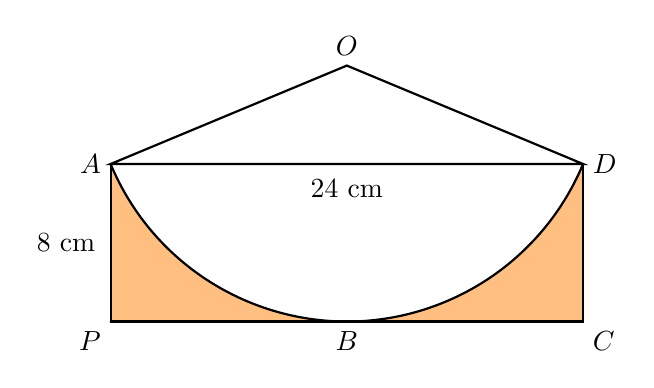
\begin{tikzpicture}[scale=0.25]
    \coordinate (O) at (0,13);
    \coordinate (A) at (-12,8);
    \coordinate (D) at (12,8);
    \coordinate (P) at (-12,0);
    \coordinate (C) at (12,0);
    \coordinate (B) at (0,0);
    \fill[orange!50] (P) -- (A) arc ({180+asin(5/13)}:{360-asin(5/13)}:13) -- (C) -- cycle;
    \draw[thick] (A) -- (O) -- (D) -- cycle;
    \draw[thick] (A) -- (P) -- (C) -- (D);
    \draw[thick] (A) arc ({180+asin(5/13)}:{360-asin(5/13)}:13);
    \fill (O) circle (1.5pt) node[above] {$O$};
    \fill (A) circle (1.5pt) node[left] {$A$};
    \fill (D) circle (1.5pt) node[right] {$D$};
    \fill (P) circle (1.5pt) node[below left] {$P$};
    \fill (C) circle (1.5pt) node[below right] {$C$};
    \fill (B) circle (1.5pt) node[below] {$B$};
    \node[below=2pt] at (0,8) {$24\text{ cm}$};
    \node[left=2pt] at (-12,4) {$8\text{ cm}$};
    \end{tikzpicture}
  \end{center}

    \begin{questionparts}
        \item 已知半径 $OA = OB = OC$,应用毕氏定理，求扇形 $OABD$ 的半径。 \qscore{4}
        \item 已知$\angle AOD = 134.76\circ$，以弧度表示$\angle AOD$。 \qscore{2}
        \item 求着色部分的面积。 \qscore{4}
    \end{questionparts}
\end{question}

\begin{solution}
    \begin{enumerate}[label=(\alph*)]
        \item \textbf{求半径：} \\
        设 $r$ 为扇形的半径，$M$ 为 $AD$ 的中点（即 $O$ 到 $AD$ 的垂足）。由对称性，$OM \perp AD$，且 $B$ 为圆弧与底边 $PC$ 的切点，故 $OB$ 亦垂直于 $PC$，$O, M, B$ 三点共线。 \\
        由切线性质，$OB = r$（半径垂直于切线）。又 $MB = AP = 8$ cm（$AD$ 与 $PC$ 之间的垂直距离），故 \\
        $OM = OB - MB = r - 8$ \hfill (1分) \\
        又 $MA = \dfrac{1}{2}AD = 12$ cm，在直角三角形 $OMA$ 中，$OA = r$，利用毕氏定理： \\
        $r^2 = MA^2 + OM^2 = 12^2 + (r - 8)^2$ \hfill (1分) \\
        $r^2 = 144 + r^2 - 16r + 64$ \\
        $0 = 208 - 16r$ \hfill (1分) \\
        $r = 13$ cm \hfill (1分)

        \item \textbf{求 $\angle AOD$：} \\
        在直角三角形 $OMA$ 中，$MA = 12$ cm，$OM = r - 8 = 13 - 8 = 5$ cm \\
        $\tan(\angle AOM) = \dfrac{MA}{OM} = \dfrac{12}{5}$ \hfill (1分) \\
        $\angle AOM = \tan^{-1}\left(\dfrac{12}{5}\right) = 1.176$ rad（4 位有效数字） \hfill (2分) \\
        由对称性，$\angle AOD = 2 \times \angle AOM = 2(1.176) = 2.352$ rad（4 位有效数字） \hfill (1分)

        \item \textbf{求着色部分的面积：} \\
        着色部分 $=$ 长方形 $APCD$ 的面积 $-$ 弓形（弦 $AD$ 与弧 $AD$ 之间）的面积 \hfill (1分) \\
        长方形面积 $= AD \times AP = 24 \times 8 = 192$ cm$^2$ \\
        弓形面积 $= \dfrac{1}{2}r^2(\theta - \sin\theta)$，其中 $r = 13$ cm，$\theta = \angle AOD = 2.352$ rad \hfill (1分) \\
        $\sin\theta = \sin(2.352) = 0.7101$ \\
        弓形面积 $= \dfrac{1}{2}(13)^2(2.352 - 0.7101) = 84.5(1.6419) = 138.7$ cm$^2$ \hfill (1分) \\
        $\therefore$ 着色部分面积 $= 192 - 138.7 = 53.3$ cm$^2$（3 位有效数字） \hfill (1分) \\
        \textbf{答：着色部分的面积约为 $53.3$ cm$^2$。}
    \end{enumerate}
\end{solution}
%endregion

%region 范围：高中数学-弧度制与扇形面积 | 考点：弧度制表示圆心角、扇形面积公式 | 难度：中等
\begin{question}[points = 6]
    已知扇形 $OAB$ 的半径 $r = 4\text{ cm}$，弧 $AB$ 的弧长 $l = 8\text{ cm}$，如图所示。

    \begin{center}
        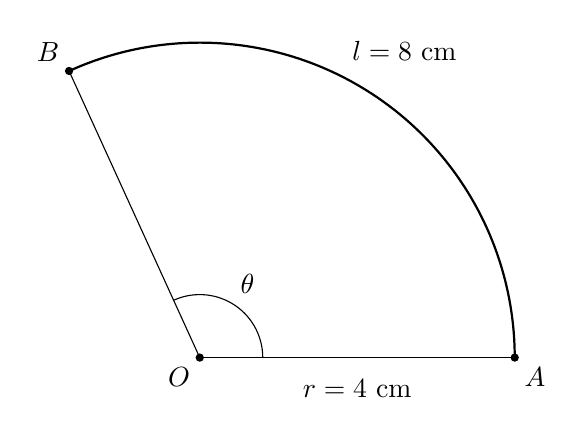
\begin{tikzpicture}[scale=1]
            \coordinate (O) at (0,0);
            \coordinate (A) at (4,0);
            \coordinate (B) at (-1.66,3.64);

            \draw (O) -- (A);
            \draw (O) -- (B);
            \draw[thick] (A) arc (0:114.59:4);

            \fill (O) circle (1.5pt) node[below left] {$O$};
            \fill (A) circle (1.5pt) node[below right] {$A$};
            \fill (B) circle (1.5pt) node[above left] {$B$};

            \node at (2,-0.4) {$r=4\text{ cm}$};
            \node at (2.6,3.9) {$l=8\text{ cm}$};

            \pic[draw, "$\theta$", angle radius=8mm, angle eccentricity=1.4] {angle=A--O--B};
        \end{tikzpicture}
    \end{center}

    \begin{questionparts}
        \item 以弧度制表示圆心角 $\theta$。 \qscore{2}

        \item 求扇形 $OAB$ 的面积。 \qscore{4}
    \end{questionparts}
\end{question}

\begin{solution}
    \begin{enumerate}[label=(\alph*)]
        \item 求圆心角 $\theta$（弧度制）。 \\
        由弧长公式 $l = r\theta$，得 $\theta = \dfrac{l}{r}$。
        \[
            \theta = \frac{l}{r}
        \]
        \hfill (1分) \\
        \[
            \theta = \frac{8}{4} = 2 \ \text{（弧度）}
        \]
        \hfill (1分)

        \item 求扇形 $OAB$ 的面积 $S$。 \\
        由扇形面积公式 $S = \dfrac{1}{2}r^2\theta$，代入 $r=4,\ \theta=2$。
        \begin{align*}
            S &= \frac{1}{2}r^2\theta \\
            &= \frac{1}{2} \times 4^2 \times 2
        \end{align*}
        \hfill (2分) \\
        \begin{align*}
            S &= \frac{1}{2} \times 16 \times 2 \\
            &= 16 \ \text{cm}^2
        \end{align*}
        \hfill (2分)
    \end{enumerate}
\end{solution}
%endregion

% %region 范围：高中数学 - 弧度制 | 考点：弧度制、扇形面积公式、弧长与周长、毕氏定理 | 难度：中等
% \begin{question}[points = 12]
%     如图所示为一等腰三角形 $OAB$，其中 $OA = OB = 15$ cm，扇形 $OCD$ 是以 $O$ 为圆心的扇形，其半径为 $10$ cm。已知扇形 $OCD$ 的面积为 $30$ cm$^2$。由 $O$ 向 $AB$ 作垂线，垂足为 $M$，且 $OM = 14.33$ cm。
% \begin{center}
%       \begin{tikzpicture}[scale=1]
%         \coordinate (O) at (0,0);
%         \coordinate (A) at (240:6);
%         \coordinate (B) at (300:6);
%         \coordinate (C) at (240:4);
%         \coordinate (D) at (300:4);
%         \coordinate (M) at (0,-5.1962);

%         \fill[orange!50] (A) -- (B) -- (D) arc (300:240:4) -- cycle;

%         \draw[thick] (O) -- (A) -- (B) -- cycle;
%         \draw[thick] (C) arc (240:300:4);
%         \draw[thick, dashed] (O) -- (M);

%         \fill (O) circle (1.5pt) node[above] {$O$};
%         \fill (A) circle (1.5pt) node[below left] {$A$};
%         \fill (B) circle (1.5pt) node[below right] {$B$};
%         \fill (C) circle (1.5pt) node[above right] {$C$};
%         \fill (D) circle (1.5pt) node[above left] {$D$};
%         \fill (M) circle (1pt) node[below] {$M$};

%         \pic[draw,"$\theta$",angle radius=8mm,angle eccentricity=1.3]{angle=A--O--B};
%         \pic [draw, angle radius=2mm] {right angle = O--M--B};

%         \draw[<->, >=latex] ([shift={(150:0.5)}]O) -- ([shift={(150:0.5)}]A) node[midway, left] {$15\text{ cm}$};
%         \draw[<->, >=latex] ([shift={(30:0.5)}]O) -- ([shift={(30:0.5)}]D) node[midway, right] {$10\text{ cm}$};
%         \node[right] at (0.15,-2.6) {$14.33$ cm};
%     \end{tikzpicture}
% \end{center}

%     \begin{questionparts}
%         \item 求 $\theta$ 之值，答案以弧度表示。 \qscore{4}
%         \item 求着色部分的周长。 (答案准确至两位小数)\qscore{6}
%     \end{questionparts}
% \end{question}

% \begin{solution}
%     \begin{enumerate}[label=(\alph*)]
%         \item \textbf{求 $\theta$ 值：} \\
%         扇形面积公式为 $\dfrac{1}{2}r^2\theta$，其中 $r = 10$ cm \\
%         $30 = \dfrac{1}{2}(10)^2\theta$ \hfill (1分) \\
%         $30 = 50\theta$ \\
%         $\theta = 0.6$ rad \hfill (3分)

%         \item \textbf{求着色部分的周长：} \\
%         $AC = DB = OA - r = 15 - 10 = 5$ cm（每段） \hfill (2分) \\
%         弧长 $CD = r\theta = 10(0.6) = 6$ cm \hfill (2分) \\
%         由于 $OA = OB$（等腰三角形），垂线 $OM$ 平分底边 $AB$，即 $M$ 为 $AB$ 中点。 \\
%         在直角三角形 $OMA$ 中，利用毕氏定理求 $AM$： \\
%         $AM^2 = OA^2 - OM^2 = 15^2 - 14.33^2 = 225 - 205.3489 = 19.6511$ \\
%         $AM = 4.433$ cm \hfill (2分) \\
%         $\therefore AB = 2 \times AM = 2(4.433) = 8.87$ cm（3 位有效数字） \hfill (1分) \\
%         $\therefore$ 周长 $= AC + \text{弧} CD + DB + AB$ \\
%         $= 5 + 6 + 5 + 8.87 = 24.9$ cm（3 位有效数字） \hfill (1分) \\
%         \textbf{答：着色部分的周长约为 $24.9$ cm。}
%     \end{enumerate}
% \end{solution}
% %endregion

\vfill % 与上方内容保持距离

\noindent
\newlength{\sigwidth}
\settowidth{\sigwidth}{（\hspace{4em}师）}

\begin{tabular*}{\textwidth}{@{\extracolsep{\fill}} l l l}
    出题： & 审题： & 审核： \\[4em]
    \rule{\sigwidth}{0.5pt} &
    \rule{\sigwidth}{0.5pt} &
    \rule{\sigwidth}{0.5pt} \\
    （\hspace{0em} \setterteacher ） &
    （\hspace{0em} \reviewteacher ） &
    （\hspace{0em} \auditteacher ） \\
\end{tabular*}


\end{document}